

% % \begin{figure}[htp]
% % \centering
% % %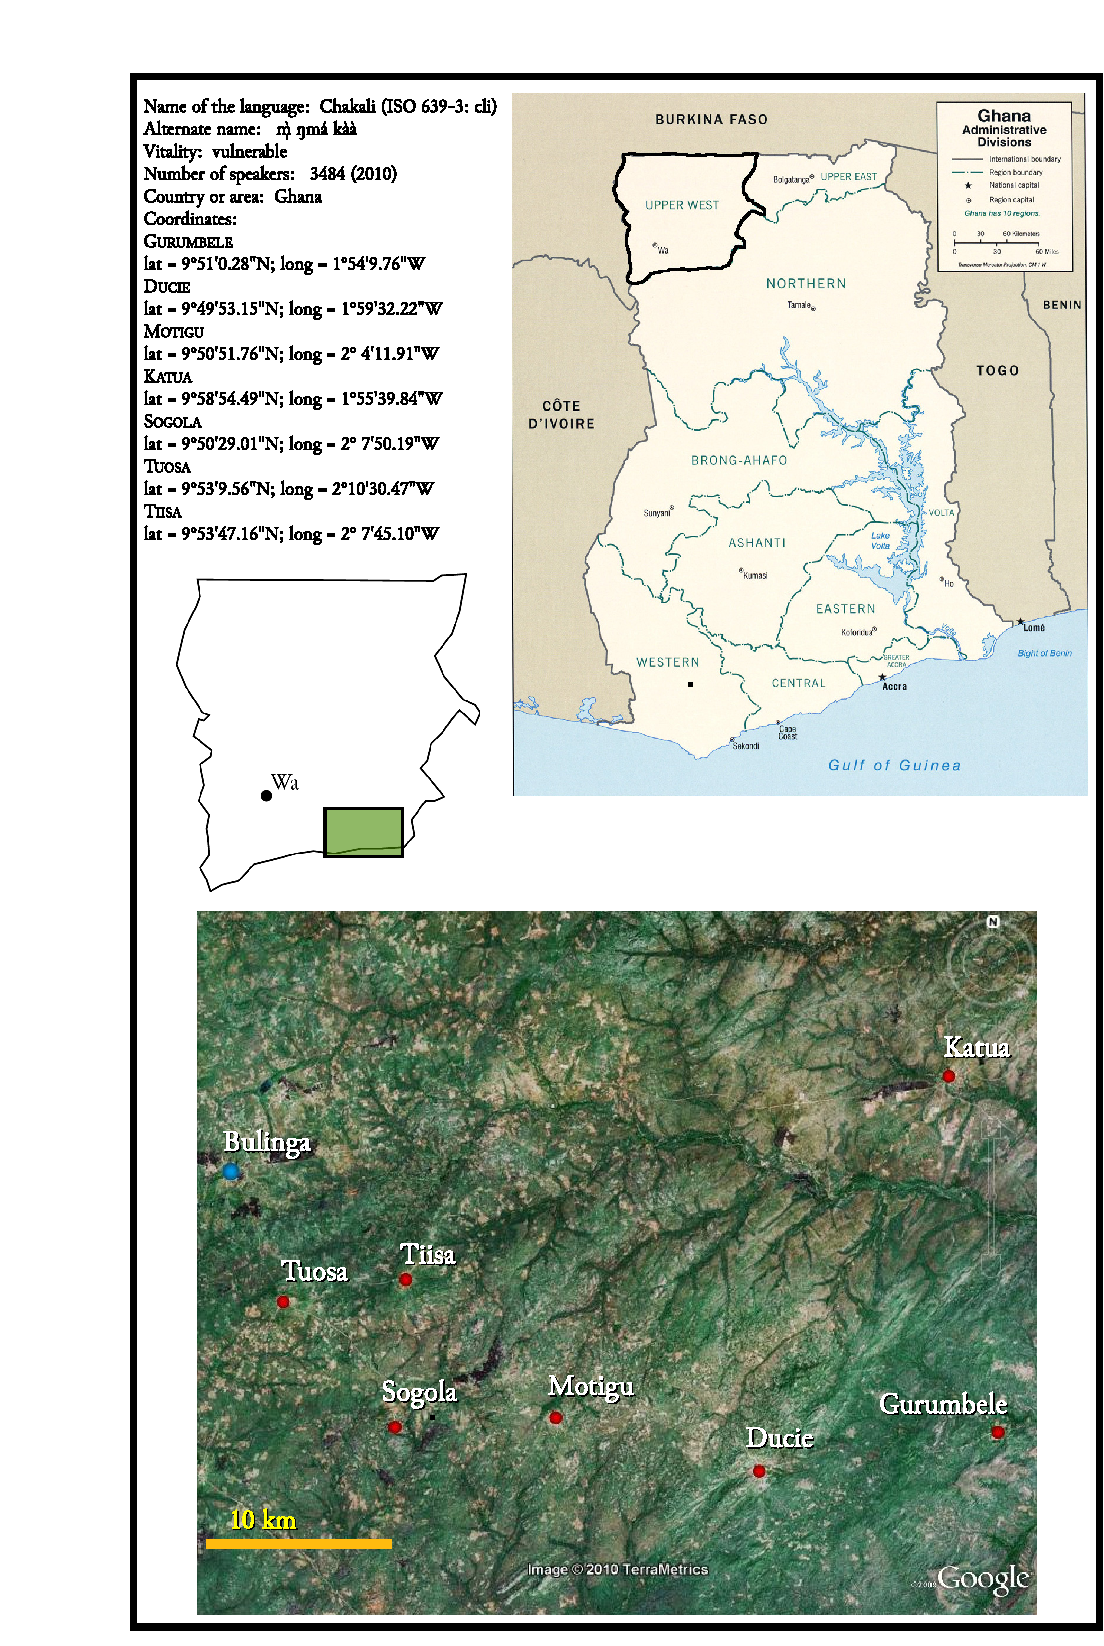
\includegraphics[height=7.2in]{Graphic/Maps/climapII.pdf}
% % 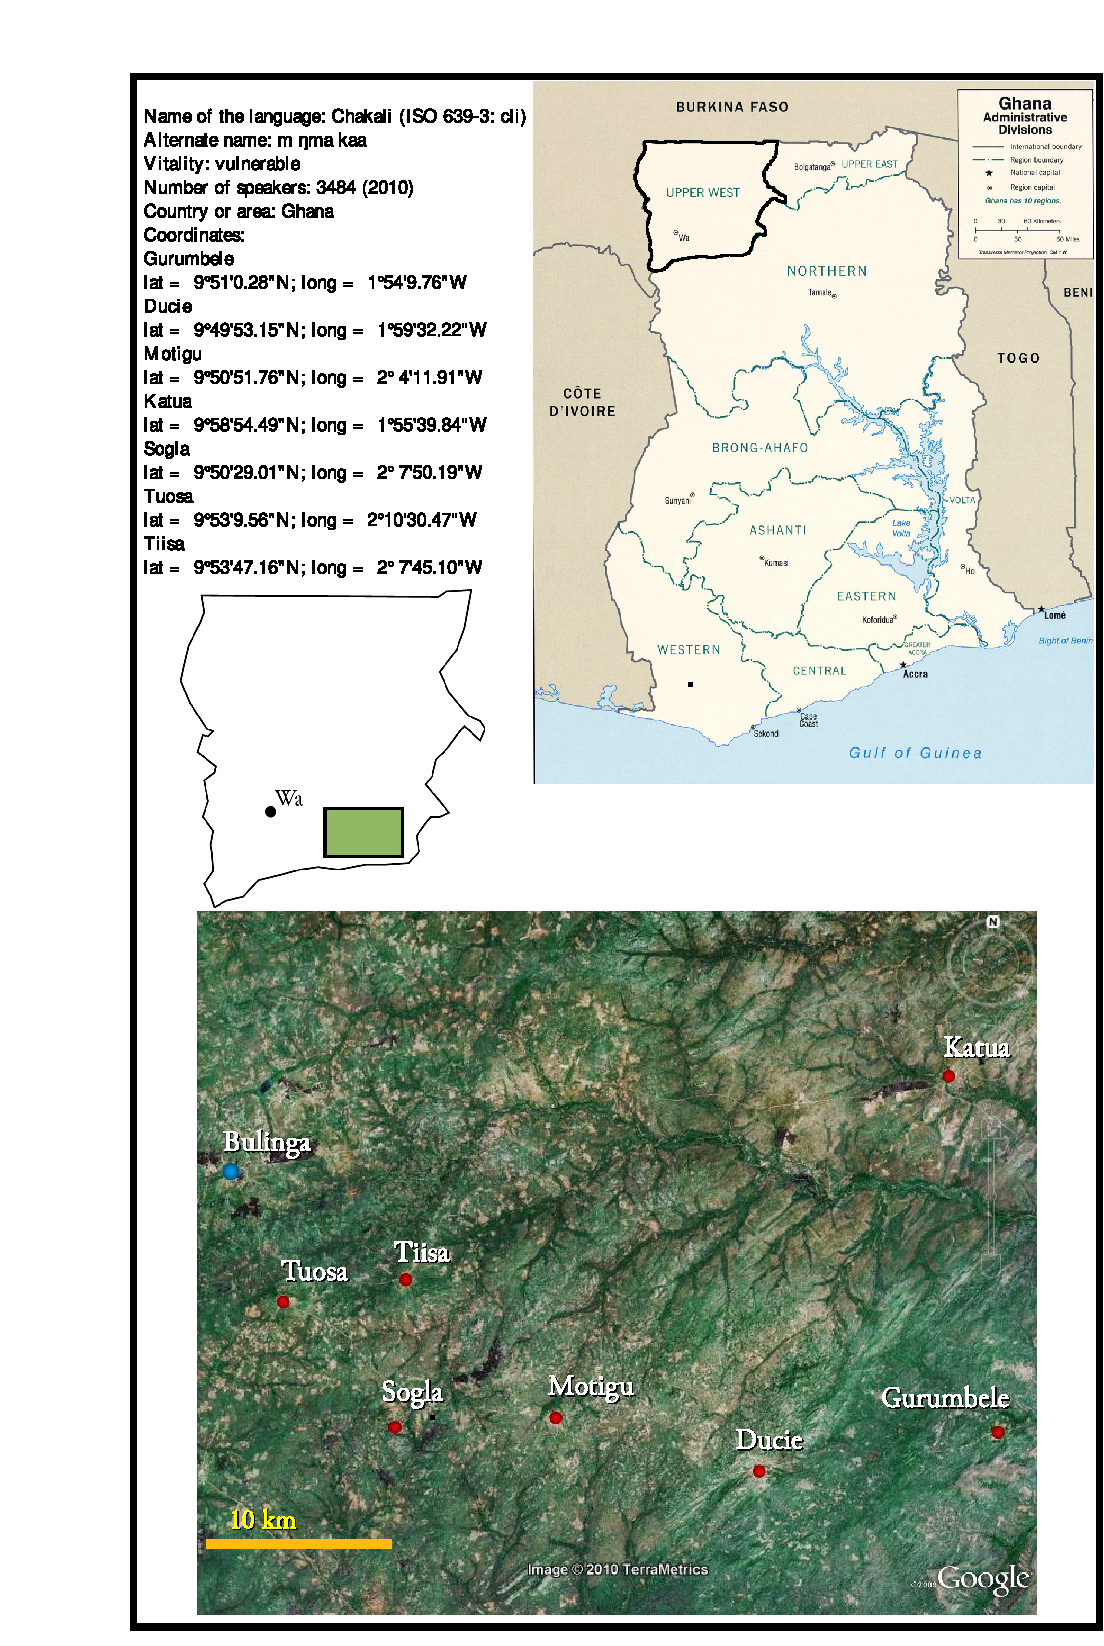
\includegraphics[clip=true, trim= 20mm 0mm 0mm 10mm, 
% % height=7.2in]{Graphic/Maps/climap.pdf}
% % % climap.pdf: 0x0 pixel, 0dpi, 0.00x0.00 cm, bb=
% % 
% % \caption[Chakali speaking area]{Chakali
% % speaking villages (Gurumbele,
% % Ducie, Motigu, Sogla, Tuosa, Tiisa and  Katua), Bulenga and Upper West
% %  regional capital Wa (Source: Google\texttrademark \   and Central Intelligence
% % Agency) \label{fig:INT-cliland}}
% % \end{figure}
% % 
% % 
% % 


\chapter{Introduction}
\label{sec:intro}

\section{General Remarks on the Language}
\label{sec:background}

Chakali  {\it (tʃàkálɪ́ɪ́)} (ISO 639-3: cli) is a language  spoken in seven 
communities in the Wa 
East District, Upper West Region of Ghana.   It is currently classified  into 
the {\it 
 \is{Grusi}Grusi Southwestern} subgroup of the Gur family, alongside with Dɛg, 
Vagala, 
Tampulma, Kyitu, Phuie, Winyé, and varieties of Sisaala \citep{lewi14, hamm14}; 
all minority languages spoken in northwest Ghana, southwest Burkina Faso,  and 
northeast Ivory Coast.  The languages  Tampulma, Vagala, Dɛg, 
and  Pasaale -- a variety of  of Sisaala --  are the closest to Chakali in 
terms 
of mutual intelligibility.

%see map

\subsection{Previous Work}
\label{sec:chrono}

The English anthropologist Jack Goody  not only  presented the first linguistic 
data on the Chakali language, which consisted of a list of 38 words gathered  
on August 29th, 1952,  in Katua \citep[33]{Good54}, but  is also 
responsible 
for the identification of the existence of the language and the people who 
speak 
it.\footnote{There may be British and/or French colonial documents somewhere 
which mention `Chakali'. For instance,  it is known that French Captain  
Louis Gustave Binger 
and his troop attacked some of Babatu's men in  Ducie.  Binger's reports were 
impossible to get hold of. \citet[133]{Wilk89} writes ``Zabarima occupation of 
Ducie occurred probably early in May 1897''.}

\begin{quote} I do not know of any previous record of the existence of the 
group speaking this dialect. Although now living entirely within the 
administrative district of Wa, there is in their midst the village of Kandia 
inhabited only by Guang-speaking Gonjas. The chiefship of Kandia was an 
important office in the Gonja political system. Either at the time of the 
arrival of the British military forces or a little before, during the course of 
a war between the State of Wa, allied with Bole, and the Yabumwura, the senior 
chief of Gonja, it fell within the orbit of Wa. The western section of the 
group 
comprising the villages of Chago, Bisikan and Bulinga speaks Wala, i.e. the 
dialect of Dagari spoken within the State of Wa, and was certainly under the 
influence of the Chiefs of Wa before the European conquest. The Chief of 
Bulinga, the central village of this section, claims to have been a Kamboŋa (a 
semi-dependent war-chief) in relation to Wa. The eastern group of the Chakalle 
speak Chakalle and seem to have been under the suzerainty of the Gonja Chief at 
Kandia. This group consists of the villages of Katua, Tosa, Sogola, Motigu, 
Chasia, Ducie and Gurembele. \citep[3]{Good54} 
\end{quote}

Approximately ten years later, Chakali data is used to confirm the 
\is{Grusi}Grusi 
cluster in \citet{Bend65}.\footnote{\is{Grusi}Grusi  as a language cluster 
has been defined and confirmed in several publications \citep{Dela12, Kohl58, 
Bend65, Mane69a, Mane69b, Klei97}, but  the term  {\it \is{Grusi}Grusi} and its 
spelling variants (i.e. {\it Gurunsi}, {\it Grunshie}, {\it Gourounsi}, etc.)  
have always existed in the French and English colonial vocabulary without great 
unanimity on its designation \citep{Taux21, Taux24, Ratt32a, Ratt32b, Nico52, 
Dupe84}. }  The material, a list of 97 words, is said to have been produced by  
Mr. E. R. Rowland.  His notes have not been located and remain unpublished.  
\citet{Mane69a, Mane69b} reconstructs  a {\it  gurunsi commun}  based on an 
average of 80 words from twenty-six \is{Grusi}Grusi languages.  He uses  
only 36 Chakali words, all of them extracted from \citet{Bend65}. In 
1974 and 1994, sociolinguistic surveys were carried out in the Chakali area by 
the Ghana Institute of Linguistics, Literacy and Bible Translation (GILLBT), 
formerly Ghana Institute of Linguistics (GIL), which is the Ghanaian branch of 
the Summer Institute of Linguistics (SIL) \citep{Reim75, Tomp02}. For these two 
surveys, the main goal  was to investigate the need of Chakali language 
development and to assess  Waali comprehension. No language data is offered in 
these surveys. In 1999, Dr. Ulrich Kleinewillinghöfer spent a few hours in Wa 
with Godfrey Bayon Tangu \citep{Klei99}. In this short period,  he  gathered 
approximately 150 words  and from them  inferred some generalizations on Chakali 
nominals. In 2001, a Brazilian  known as Pastor Ronaldo worked with two  
language consultants in order to start a vernacular literacy project. The 
initiative came from the Evangelical Church of Ghana.  Two illustrated booklets 
were written,  aiming at adult literacy.  The first 
booklet introduces the designed alphabet  and the second  
consists of  syllables and short sentences thematically organized. In 2005, 
Prof. Mary Esther Kropp-Dakubu spent two  days with an informant from Jayiri, 
gathering general information on Chakali  \citep{Daku05}. Her intention was to 
investigate the situation on site for a possible documentation project. Due to 
the 
condition of the road, she did not reach villages where Chakali is spoken by the 
majority of the inhabitants.  Her unpublished report  presents  data which was 
believed to be representative of  Chakali, but which transpired to be an 
idiosyncratic mix of Waali and Chakali, and some Bulengi,  a language spoken in 
Bulenga and surrounding villages. 
Finally, there are other studies that deserve to be
mentioned:  Dr. Henry Seidu Daannaa,   a native Chakali from Tuosa,  presents a
retrospective study of the practice of indirect rule  which affected the
social and political organization of  Chakali during the colonial 
administration 
\citep{Daan94};    Dr. Cesare Poppi conducted anthropological research which 
focused on issues related to knowledge, secrecy,  and initiation 
\citep{Popp93}, 
and  theoretical issues concerning the analysis of the representational status 
of masks, particularly the {\it Sigmaa} masks which are cornerstones in the  
Chakali 
belief system; the work of \citet{Doug66},  \citet{Wilk89}, and \citet{Sali08}  
are good  overviews 
on 
the role of the Chakali land and people in the  political and cultural history 
of Wa.

This section has offered a complete list of work written on Chakali. It shows 
that the language has been 
known to exist since 1954, yet very little work has been done,  and  most of 
what 
has been written  remains unpublished.

\subsection{Chakali Lects}
\label{sec:lects}

With Chakali,    three concepts can be
identified. The term may be used  to name a land,  
an ethnic group,   or a language.  
However it would be wrong to assume that a member of the Chakali ethnic group  
or 
 someone living in Chakali land necessarily speaks the language.  This is 
 what \citeauthor{Good54} describes: 

\begin{quote} [t]he use of one self-applied name may cut across the linguistic
frontiers which have already been defined. The Chakalle who inhabit the eastern
part of the Wa district are split into those speaking a language of the Mossi
group and those speaking a \is{Grusi}Grusi language. ``Speaking a language" 
refers to the
tongue which dominates in the child's play group; the eastern Chakalle who use a
\is{Grusi}Grusi language in this context are in fact mostly bilingual. The 
common name for
the group derives from a recognition of uniformity in other social activities.
  \citet[2]{Good54}
\end{quote}
 
 

\begin{figure}[htp]
\centering
%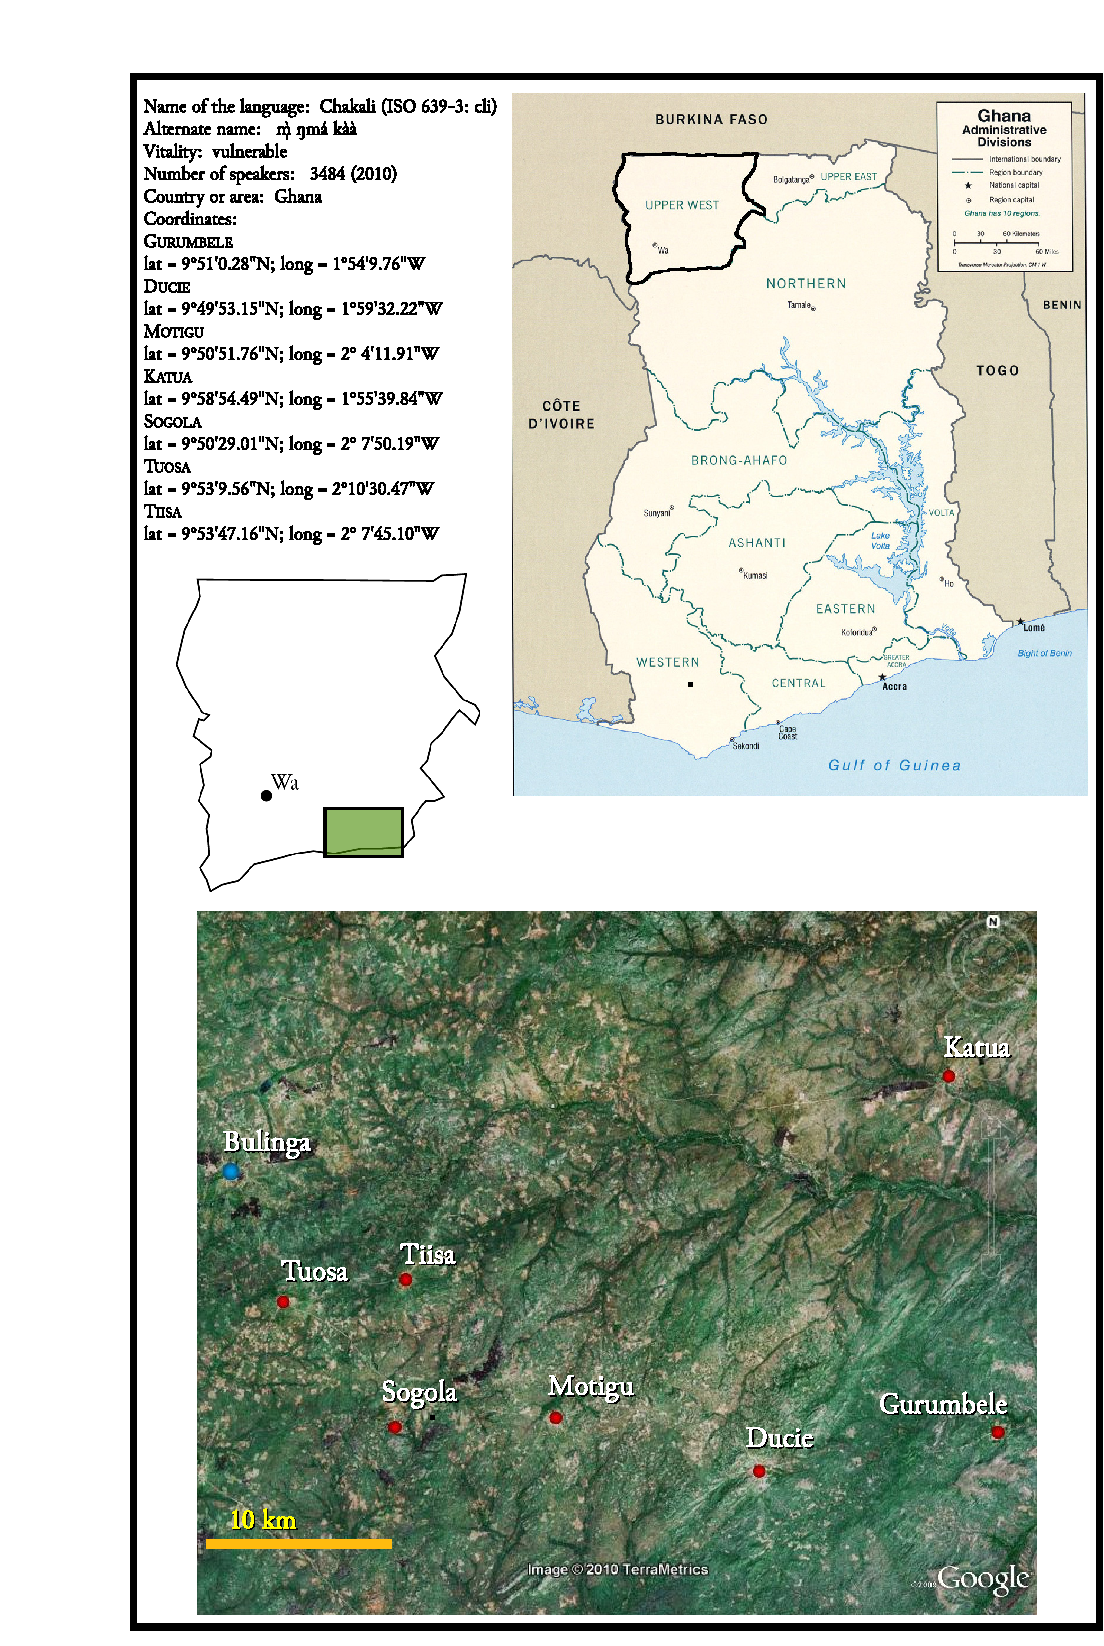
\includegraphics[height=7.2in]{Graphic/Maps/climapII.pdf}
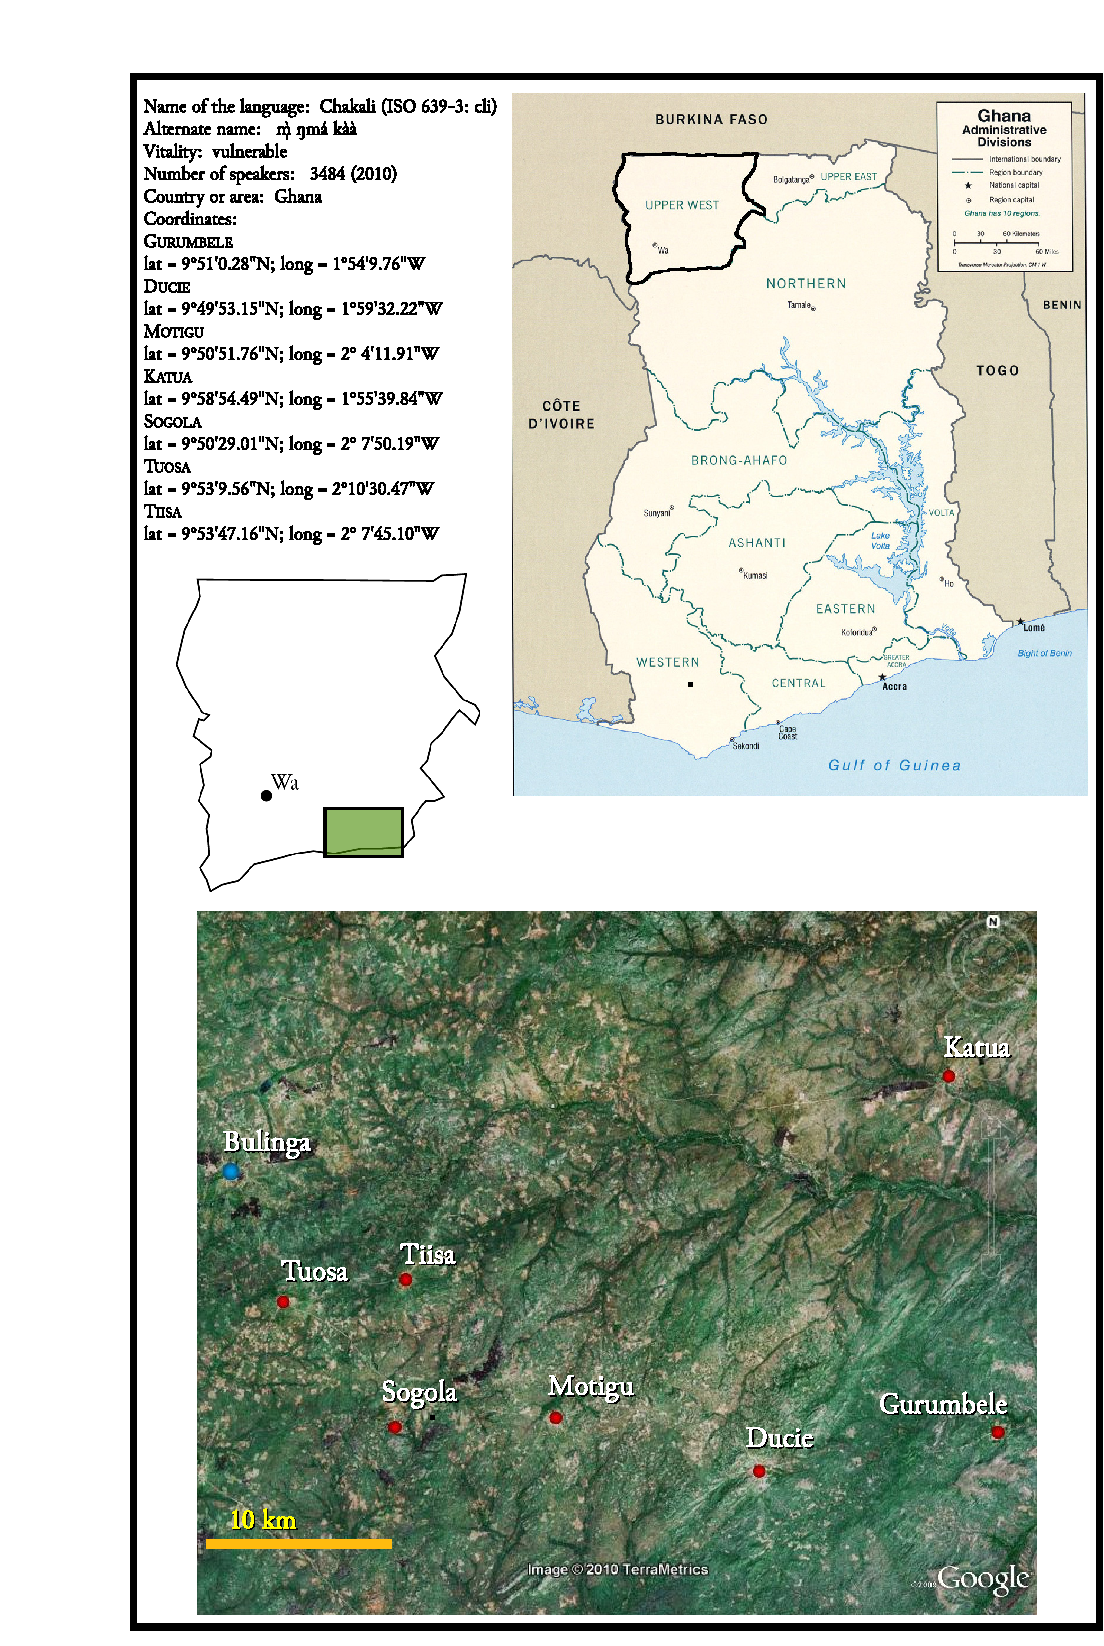
\includegraphics[clip=true, trim= 20mm 0mm 0mm 10mm, 
height=6.6in]{Graphic/Maps/climapII.pdf}
% climap.pdf: 0x0 pixel, 0dpi, 0.00x0.00 cm, bb=

\caption[Chakali speaking area]{Chakali
speaking villages (Gurumbele,
Ducie, Motigu, Sogla, Tuosa, Tiisa and  Katua), Bulenga and Upper West
 regional capital Wa (Source: Google\texttrademark \   and Central Intelligence
Agency) \label{fig:INT-cliland}}
\end{figure}

\begin{sidewaysfigure}
 \centering

\includegraphics[height=4.8in]{Graphic/Maps/project-4.jpg}
% climap.pdf: 0x0 pixel, 0dpi, 0.00x0.00 cm, bb=

\caption[]{Caption\label{fig:}}
\end{sidewaysfigure}


 

 
It is crucial to keep in mind that these three concepts (i.e. land, 
ethnicity, and language) are interwoven.   For instance, according to 
\citet{Daan94},  {\it Chakali}  consists of  thirteen communities 
and 
their inhabitants:  Bulenga, Tiisa, Sogla, Tuosa, Chagu, Motigu, Ducie, Katua, 
Bisikan, Kandia, Dupari, Gilan and Gurumbele.  By contrast, the 
sociolinguistic 
censuses which I carried out indicate that {\it Chakali} is the 
language 
of the inhabitants and forefathers of  Tiisa, Sogla, Tuosa,  Motigu, Ducie, 
Katua, and  Gurumbele exclusively.


The \is{demonym}demonym for the people of these seven villages literally 
translate to  
{\it m̩̀ ŋmá kàà} {\it (lit.)}   `I say that',  whereas that of  the 
people 
of Bulenga and surrounding villages translate to   {\it ŋmɪ́nɪ́ŋ dʒɔ̀ŋ}  `What 
is it?'.   In this folk-sociolinguistic categorisation, the Waala are the {\it 
ǹ̩ jɛ́ jàà} `I say that'.\footnote{\citet[525]{Ratt32b} writes that the 
Awuna,  a Kasem dialect also known as Aculo \citep[147]{Nade89},  has earned 
its 
appellation based on a habit of  ``prefacing an observation with the words''  
{\it a wun a} `I say'. It is indeed the case that a Chakali  can open a sentence 
with {\it m̩̀ ŋmá kàà, ...}  `I say that, ...'. To hear the  Ghanaian 
English opening 
expression {\it à sé ɛ̃̀ɛ̃̀}  `I say eh, ...'   in Wa town is not 
unusual.}   Another popular distinction  is that of `black' and `white' 
Chakali;  respectively, the eastern block is the {\it tʃàkàlbúmmò} `Black 
Chakali',  a notion which connotes  secretive individuals, possessors of 
powerful medicine. I was told that Tuosa and Tissa are not part of the `Black 
Chakali'.   The western block is  the   {\it tʃàkàlpʊ̀mmá}  `White Chakali', 
i.e. people who are talkative and cannot hold back.\footnote{This comes from 
my 
`Black Chakali' consultants. Obviously, if one asks the same question in Bulenga 
and surrounding villages one may get a different interpretation of the 
distinction.}  This way of making a distinction 
between linguistic groups corresponds more or less to what \citet[2-3]{Good54} 
calls eastern Chakali and Western Chakali. Within the 
{\it m̩̀ ŋmá kàà}, there 
exist lexical, phonological, and prosodic variations which validate 
folk-dialectology. The lect of Katua, Tiisa and Tuosa,  on one hand, and the 
lect of Ducie and Gurumbele, on the other hand,  are considered the farthest 
apart on a continuum.\footnote{A Sogla-Motigu lect   could be situated somewhere 
in the middle of such continuum. One version of the migration and creation of 
Katua, Tiisa,  and Tuosa is presented in \citet[74-82]{Sali08}.} Examples 
of lectal variation are provided in \citet{brin15c}, but one recurrent 
illustration of folk-dialectology  is  how each village would express `to 
eat yam':   Motigu, Gurumbele, Tuosa, Tiisa,  and Katua  `chew' yam {\it 
(tie)}, 
whereas Ducie  `eat' yam {\it (di)}.  And while `yam' is pronounced {\it 
kpããŋ} in Motigu, Gurumbele,  and Ducie, it is pronounced {\it pɪɪ} in Tuosa, 
Tiisa,  and Katua. Thus, if someone says {\it tie kpããŋ}, he/she is 
easily identified as someone from either Gurumbele or Motigu.  The expression 
{\it di kpããŋ} is typically uttered by someone from  Ducie,  and {\it tie pɪɪ} 
by someone from Tuosa,  Tiisa, and Katua.  Still, each village is recognised to 
have a set of unique features. For instance, within the Ducie-Gurumbele lect, 
Ducie people consider that {\it Bɛ̀lɪ́lɪ́ɪ́}, the Gurumbele lect,  is a lect 
resembling a mixture of {\it Dùsélíí}, the lect of Ducie, and the lect 
of Gbanwale {\it (gbúŋwálɛ́)}, i.e. a variety of Tampulma. They also say that 
the Gurumbele lect is ``stretched'', and that the speakers ``pull their 
words''. The 
people of Gurumbele believe the opposite, saying that Ducie lect  is 
 ``short''.  These statements are  reported in (\ref{ex:SOC-bele-duc-lect}). 



\begin{exe}
 \ex\label{ex:SOC-bele-duc-lect}
\begin{xlist}
 \ex\label{ex:SOC-bele-lect}
\gll bɛ̀lɪ́lɛ́ɛ́ tàá tɪ̀ŋ ʊ̀ já tátʊ́ʊ̀\\
lect.type language {\art} {3\sg} {\sc hab} pull.{\foc}\\
\glt `The language of Gurumbele; it pulls/stretches.'

 \ex\label{ex:SOC-ducie-lect}
\gll dùsíéléé tàá tɪ̀ŋ ʊ̀ jáá bòrò rò\\
lect.type language {\art} {3\sg} {\ident}  short {\foc}\\
\glt `The language of Ducie; it is short.'
\end{xlist}
\end{exe}

Despite the above linguistic and anecdotal facts reporting the presence 
of variations,  all the Chakali lects are mutually intelligible.


\subsection{Language Vitality}
\label{sec:vital}

The number of Chakali speakers is close
to 3500 individuals. It is spoken by all community members in Gurumbele and 
Ducie, and by
the majority in Motigu and Katua. It is spoken to a lesser extent in Sogola,
Tuosa,  and Tiisa.  In the other villages which are considered as  parts of
Chakali land, people speak a language similar to Waali, the language of  Wa, or
Bulengi, the language of Bulenga. Waali is known by the majority of Chakali
speakers,  but is used differently from community to community.   Chakali is 
believed
to be on the road to extinction: some believe that Waali and Bulengi are the
languages which will be spoken throughout the whole of the Chakali villages in 
the
coming decades.



\begin{sidewaysfigure}
\footnotesize
  \centering
 \begin{tabular}{p{5cm}p{3.5cm}p{3.5cm}p{3.5cm}}


 %\begin{Atabular}{ll}
\toprule
    Factors & \multicolumn{3}{c}{Measures}\\[1ex]\midrule
 &E1&E2&E3\\[1ex]\midrule

1. Intergenerational language transmission &  {severely endangered} 
(2) & {unsafe} (4)& {safe} (5)\\

2.  Absolute number of speakers  &
\multicolumn{3}{c}{[{ 3484}]}\\ 

3. Proportion of speakers within the total population &
\multicolumn{3}{c}{[{severely
endangered}  (2) ]}\\

4.  Trends in existing language domains & {highly limited domains}
(2)& {dwindling domains} (3)&{multilingual parity} (4)\\

5.  Response to new domains and media& & [{
inactive-minimal}
(0-1)]& \\


6.  Materials for language education and literacy & 
\multicolumn{3}{c}{[{no orthography available} (0)]}\\

7. Governmental and institutional language attitudes
and policies, including official status and use &
\multicolumn{3}{c}{[{active
assimilation} (2) ]}\\


8. Community members attitudes toward their own language &-&-&{all
members value their language and wish to see it promoted} (5) 
\\

9.  Amount and quality of documentation &
\multicolumn{3}{c}{[{undocumented-inadequate} (0-1) ]}\\


\bottomrule
  \end{tabular}
  
\caption[Estimated degree of endangerment for the E1, E2 and E3 
villages]{Estimated degree of endangerment for the E1 \{Tuosa, Tiisa, Sogla\}, 
E2 \{Katua, Motigu\} and E3 \{Gurumbele, Ducie\}. A value within square brackets 
 applies to E1, E2 and E3 villages as a whole. The number in parentheses is a 
relative grade used in the  language vitality assessment  
\citep[see][7]{Reco03}} \label{tab:estimate-endangerment}

\end{sidewaysfigure}




 \citet{brin15c} determines the vitality of  Chakali using the 
questionnaire developed in 
\citet{Reco03} and  suggests a division of the Chakali
villages into three groups, which are presented in Figure 
\ref{tab:estimate-endangerment}. 
Sogla,
Tiisa,  and Tuosa correspond to the villages where the intergenerational
transmission is ineffective and where Waali is used in formal and informal
domains. They are the endangered-1  villages (E1).  Motigu and 
Katua correspond to 
E2
villages. In both villages,  Waali is encroaching on  Chakali in
formal and informal domains. The situation is not alarming since Chakali is
spoken by the majority and  the intergenerational transmission is effective, but
given the average population size of the villages and the recent conversion to
Islam of their youth, among other factors, it is worth considering that a 
language shift to Waali may
take place within a short period of time.  A. B. Sakara and H. S. Daanaa, both 
born in
Tuosa, told me that Chakali was spoken by everyone in their village when they
were children, i.e. in the 1950s and 1960s. There  are no signs indicating that 
the same 
language replacement which took place in Tuosa  cannot take place in Motigu and
Katua. Finally, the E3 villages, Gurumbele and Ducie, show the most effective 
intergenerational transmission of the Chakali language. Both villages also 
establish local alliances (i.e. marriage, common shrines, one assembly man for 
both villages, etc.). Waali is spoken and understood, yet it is usually spoken 
in specific  domains, for instance  in official visits from the district or 
regional capital conducted by governmental bodies,  and  to  Waali-speaking 
visitors, traders,  or migrant farmers.


\subsection{Data Collection Method}
\label{sec:lects}

Each year since 2007 I  made a field trip to the Wa East District of Ghana, 
usually in the dry season, i.e.  a  period between February and  May.  Most of 
my stays were spent in a Chakali-speaking village. I had several overnight stays 
in Motigu, Gurumbele,  and Wa, and a few day trips to Katua, Tiisa, Tuosa, and 
Sogla. The linguistic data was gathered mainly in Ducie, and sociolinguistic 
surveys were conducted in Katua, Motigu, Sogla, Ducie and Gurumbele.  



Different elicitation techniques were used to gather words and sentences.  The 
most authentic and
natural data comes from impressionistic auditory transcription of transactions 
at the market, meetings 
with the elders,  and interviews with commoners. In these cases wordlists were 
created out of the transcriptions. The least natural data are pieces of 
translation work  or exchanges of information with consultants of the type `how 
do you say X', where X stands for an intended entity or proposition, using 
English or Chakali as the medium of communication. Translations from English to 
Chakali and 
from Chakali to English  were performed through a  collaboration with 
 my main consultants, namely: 
Daniel Kanganu Karija (male, 58 Y.O., Ducie), Fuseini Mba Zien (male, 54 Y.O., 
Ducie), Awie Bakuri Ahmed (male, 31 Y.O., 
Gurumbele), and Afia Kala Tangu 
(female, 34 Y.O., Ducie). Quantitative studies required at times as many as 
50 different speakers, all of them from Ducie. The results of some of these 
studies are reported in  
\citet{BrinAtin12, brin16}.

Another method of 
elicitation 
consisted of having a significant number of native speakers interpreting,
identifying and expressing perceived stimuli.  Stimulus-based data collection
has the advantage of being free from interference and provides the researcher
with a level of authenticity unattainable in (bilingual) elicitation of
paradigms
and wordlists.  Since the data collection was carried
out with several individuals, the degree of consensus within the responses can
be interpreted as signalling core, secondary, or `accidental'
meaning. The same method is useful in practical lexicography work
when the discovery procedure involved  taxonomies unknown to the researcher. For
instance, the domains of animals and plants required the identification of
species and their associated pronounciation. A problem arises when the visual
access to some species  is practically
impossible, e.g.   hyenas or seasonal plants. While working on  the 
lexical database, many species were identified using
illustrations. One disadvantage often encountered with this approach to lexicon
and
grammar discovery is that standard stimuli  face
the problem  of cross-cultural applicability.  In the context of  northern 
Ghana, unfamiliar items or scenes depicted may cause
disagreement in
the overall description, if not confusion.  
Another obstacle is that pictures and illustrations may lack 
elementary features, such as texture, odour, size, etc., 
which are crucial for
 the identification of a species.  For
instance,
since  only  illustrations and pictures found in \citet{Cans61, Trap06} were 
used,  arriving at a consensus when identifying  
species of snake has proved difficult.   Therefore,  I believe I used the most 
satisfactory data collection strategy in such research context. Needless to say 
every piece of Chakali data in this book comes from my own transcription of 
speech. 
 
 
 


\section{User's Guide}
\label{sec:cont-descr}

At a macrostructure level, the Chakali-English dictionary is followed by the 
English-Chakali reversal index.  They contain information extracted  from a  
lexical database which I started   in 2007 using the software {\it Field 
Linguist’s Toolbox}  and imported in {\it Language Explorer (FLEx)} in  2012.  
The entries appearing in the dictionary are made out of  only a selection of  
the lexicographic fields and values available in the lexical database.

The passage from unwritten to written has the inevitable consequence of 
favouring a dialect. Any native speaker of Chakali would easily identify that 
Ducie was the community where the majority of the data was collected.  
Corresponding expressions from other varieties of Chakali are present, when they 
exist,  but more work is definitely needed.   Addressing the issue of convention 
and standardisation will require a  group of devoted contributors from distinct 
communities. There is no reason to treat the decisions taken in this book, 
especially regarding the orthography,  as the standard. It is advised to keep in 
mind that orthographic consistencies  and English translations and definitions 
are always challenging. 


% % It is valuable to identify lectal and generational variations, such as,
% % expressions used in one village but not in another and obsolete
% % expressions representative of the oldest generation. Other deficiencies 
% % in the 
% % current version are the
% % inadequate description of forms and functions in the verbal domain, of which
% % prosody is crucial in determining aspectual distinctions. 



\subsection{Chakali-English Dictionary}
\label{sec:cli-eng-entry}



The Chakali-English dictionary consists of over 3200 Chakali 
\is{headword}headword 
entries (a.k.a. \is{lemma}lemmas).
The transcription employs the 
orthography described in Chapter \ref{sec:chap-phono}.  It uses a Latin 
alphabet 
supplemented 
with symbols from the International 
Phonetic Alphabet (IPA), so the spelling-sound correspondence is direct.  A 
full list of the 
orthography symbols used in the dictionary and some guidance to their 
pronunciations are displayed in Table \ref{tab:orth-symb}.

\begin{table}[h]
  \caption{Orthography and other symbols\label{tab:orth-symb}}
\small
 \begin{tabular}{llll}
p & voiceless bilabial plosive & w&labio-velar approximant\\
b & voice bilabial plosive &j & palatal approximant \\
t & voiceless alveolar plosive &r & alveolar trill/flap\\
d &  voiced alveolar plosive&o& close-mid back rounded\\
k & voiceless velar plosive  &ɔ& open-mid back rounded\\
g & voiced velar plosive &e& close-mid front unrounded\\
ʔ & glottal stop &ɛ& open mid front unrounded\\
kp & voiceless labio-velar plosive &u& close back rounded\\
gb & voiced labio-velar plosive&ʊ& near close near back rounded\\
f & voiceless labio-dental fricative &i& close front unrounded\\
v & voiced labio-dental fricative  &ɪ& near close near front unrounded\\
s & voiceless alveolar fricative &a& open front unrounded\\
z & voiced alveolar fricative &ə& mid central\\
ɣ & voiced velar fricative&$[$ $]$ & phonetic representation\\
h & voiceless glottal fricative & ː & emphasis over or long segment\\
tʃ & voiceless postalveolar affricate & V̆ & extra short vowel\\
dʒ & voiced postalveolar affricate&C̩& syllabic consonant\\
m & bilabial nasal &  Ṽ & nasalized   vowel\\
n & alveolar nasal& V̀ & low tone \\
ɲ & palatal nasal &  V̄ & high tone \\
ŋ & velar nasal& V́ & high tone \\
ŋm & velar-labial nasal&V̏  & extra-low tone \\
l & alveolar lateral approximant  & &\\
\end{tabular}

 \end{table}
 
 

For users accustomed to the literacy work of GILLBT\footnote{Reference is made
to the literacy work on Vagla,  Tampulma, and Pasaale  of Marjorie 
Crouch\dag, Patricia Herbert, Noah Ampen, Kofi
Mensah,
Mike Toupin, Vicky Toupin, Ian Gray,  and Claire Gray.} the correspondences
in Table \ref{tab:corr-our} identify the differences between their 
transcriptions and mine. The
transcription adopted in this dictionary  appears to the right side of the 
arrows. 


\begin{table}[h]
\caption[]{Correspondences of orthographies\label{tab:corr-our}}
 \begin{center}
\framebox[3in]{
\begin{tabular}{lllllll}
% ng &$\leftarrow$& ŋ  & \hspace*{5ex} y&$\leftarrow$& j\\
ny &$\leftarrow$& ɲ  &\hspace*{5ex} Vh&$\leftarrow$&  Ṽ \\
ch  &$\leftarrow$& tʃ  &\hspace*{5ex}  i&$\leftarrow$&ɪ, i\\
j &$\leftarrow$&dʒ  &\hspace*{5ex}  u&$\leftarrow$& ʊ, u \\
y &$\leftarrow$&j  &\hspace*{5ex}  &&
\end{tabular}  
}
\end{center}
\end{table}



The headwords  are structured alphabetically  although an arbitrary decision was 
taken to place the letter `{\it  dʒ}' after `{\it  d}', `{\it  gb}' after `{\it  
g}', 
`{\it  kp}' after `{\it  k}',  `{\it  ɲ}'  and `{\it  ŋm}' successively after 
`{\it  n}',  
and `{\it  tʃ}' after `{\it  t}'.  All headwords are equal and appear at the 
left 
side of the column. Three representative entries of the Chakali-English 
dictionary are presented in Table \ref{tab:illu-dict}.\footnote{The circled 
numbers are there for reference purposes only.}

\begin{table}[h]
\caption[]{Illustrations of the Chakali-English dictionary 
entry\label{tab:illu-dict}}
 \begin{center}
\framebox[4in]{
\begin{tabular}{p{9cm}}
% \Circled{1}{\it  fi} \Circled{2}[fí]  \Circled{3}{\itshape num}.
\Circled{5}ten \\[1ex]

\Circled{1}{\it   bʊzaal}  \Circled{2} [bʊ́záàl] \Circled{8}cf: 
bɪɪzimii. \Circled{3}n.   \Circled{5} Stone partridge, type of bird  
\Circled{9}{\it 
Ptilopachus 
petrosus}   \Circledd{10} Pl: bʊzaalɛɛ \\[1ex]

\Circled{1}{\it   kpa}  \Circled{2}[kpà] 
\Circled{8}cf: paa; cf: jʊʊ$_{1}$. \Circled{3}v  \Circled{4}1) \Circled{5} take 
 
\Circled{6}kpá à pár tɪ̄ɛ̄ŋ. \Circled{7}Give me the hoe.  
\Circled{4}2) \Circled{5} to marry a woman \Circled{6}  ʊ̀ kpáʊ́ rà.  
\Circled{7}He married her

\end{tabular}
}
\end{center}
\end{table}


An entry starts with a  headword (\Circled{1}), which is immediately followed by 
its phonetic representation (\Circled{2}). This representation adds tones and 
other information on the pronunciation. Words which do not bear tones in the 
phonetic representation field are considered as either toneless or  unresolved. 
The grammatical category (\Circled{3}) provides  the word class of the headword. 
Open class items, i.e. nouns and verbs,  are the most frequent. A plural form  
is provided for the majority of the nouns \Circledd{10}. Cross references  
(\Circled{8}) appear before the part-of-speech and after the phonetic form. A 
type of variations to which different spellings or form have to be assigned is 
placed after the phonetic form. 


The meaning  is represented in the following way: if the headword has only one 
sense,  the part of speech immediately precedes the English definition 
(\Circled{5}).  If the headword has more than one sense,  a number followed by a 
right parenthesis (\Circled{4}) enumerates the different senses. When Chakali is 
translated into English using many expressions, these are separated by a comma. 
If a word typically collocates with a concept, this is expressed within  
parentheses in the English translation.  An example of usage (\Circled{6}) 
precedes its English translation (\Circled{7}). If literal and/or not easily 
translatable, this translation contains a parenthesis with clarification.

\subsubsection{Prosody}
\label{sec:INT-prosody}

The examples are all marked with diacritics which represent the prosody as I 
perceived it during the transcription work. A  short description of tone and 
intonation is provided in Section \ref{sec:tone-intonation}. At this stage, the 
transcription and description of tone will require an analysis of considerable 
sophistication, something which deserves a separate study. The convention for 
marking tone is:  high (  ́), low (  ̀), mid   (  ̄),  and super-low ( ̏ ).  
There are several issues linked to doing the transcription by ear and lacking a 
convention. For instance, due to the general downdrift,  the prosody on 
single words are easier to represent with the diacritics compared to longer 
expressions.

\subsubsection{Scientific name}
\label{sec:INT-sci-name}

To  add the referential stability needed for future comparison between
traditional  and scientific  taxonomies, scientific names appear in italics  
(\Circled{9}).   References to scientific
names of  plants and trees were taken from 
\citet{hawt06},  of  snakes from \citet{Cans61}  and \citet{Trap06}, and of  
birds 
from \citet{borr02}.




\subsubsection{Grammatical category}
\label{sec:INT-other-lex-field}

The grammatical categories (a.k.a  word classes or parts of speech)  used in the 
dictionary are all described in Section \ref{sec:gramsketch}. They are 
distinguished using distributional and inflectional criteria. Table 
\ref{tab:dict-abb} offers a  list of the sections in the grammar outline where 
each grammatical  category can be found, together with their dictionary 
abbreviation.


% \begin{table}[h]
%  \caption{Grammatical Categories and Sections\label{tab:}}
%   \centering
%   \begin{tabular}{llll}
% \lsptoprule 
% Grammatical Category & Abbreviation & Section \\
% article & 
% noun & {\itshape n} &  \\
% 
% 
%  \\
% \midrule
% 
%     
% \lspbottomrule
%   \end{tabular}
% \end{table}

% 
% verb ({\itshape v}),% 
% qualifiers ({\itshape qual}) 
% and quantifers  ({\itshape quant}), which modify 
%  nouns in  noun phrases,  adverbs  ({\itshape adv}) , which modify  verb phrases
%  or  clauses,  articles ({\itshape art}), which combine with a noun to indicate
%  the type of reference being made, classifier  ({\itshape clf}), which
%  is a selectional prefixed onto property denoting expressions and classify the
% referent either as human, concrete-(non)aninmate or abstract, relational noun
% ({\itshape reln}), which designates
% a locative search domain of an object,
% postposition ({\itshape postp}),  which signals that the
% constituent in which they appear is locative, ...
% 
% ,connective
% ,complementizer
% ,complex verb
% ,demonstrative
% ,focus
% ,ideophones
% ,interrogative
% ,interjection
% ,imperative
% ,iteratif
% ,negation
% ,numeral
% ,onomatopea
% ,postposition
% ,reciprocal
% ,reflexive
% ,tam
%


\subsubsection{Loans and their etymology}
\label{sec:INT-loan-ety}


Loan words are given a source and when necessary the source's pronunciation and 
gloss. Some are well-established, and others are intuitive. As the sources are 
not 
always easy to identify, some are followed by a question mark. I  put the 
word  {\it ultimately} (abbreviated {\it ultm.}) prior to the source language
to mean that the loan word might not have been borrowed directly from the 
speakers of the language with which the word is associated. For example, it is 
most likely that all English words entered Chakali  through contact with 
speakers of other Ghanaian languages.  Section \ref{sec:GRM-borr-noun} offers an 
overview of languages from which Chakali may have borrow.  References to 
etymologies are mainly taken from \citet{newm07hausa}, \citet{daku07},  
\citet{daku09ga},  \cite{vagl80},  and  \citet{Dume11}.


\subsection{English-Chakali Reversal Index}
\label{sec:eng-cli-entry}

The English-Chakali reversal index is a list of  alphabetically organized 
English headwords (\Circled{1}). As shown in Table 
\ref{tab:illu-index}  the headword may be 
associated with  more than one  Chakali 
gloss entry (\Circled{5}).  



\begin{table}[h]
\caption[]{Illustration of the English-Chakali reversal 
index entry\label{tab:illu-index}}
\begin{center} 
\framebox[3in]{

\begin{tabular}{lll}
 \Circled{1}grasshopper (type of) & \Circled{3}{\itshape n.} & 
\Circled{5}{hɔ̃ʊ̃} \\
 & \Circled{3}{\itshape n.} & \Circled{5}{tʃɛlɪntʃɪɛ} \\
 & \Circled{3}{\itshape n.} & \Circled{5}{kɔkɔlɪkɔ} \\
\end{tabular} 
}
\end{center} 
\end{table}



English  headwords are reduced to 
minimal terms in order to have the index easily searchable. 
Several English expressions can be associated with one Chakali word: for 
instance, 
all Chakali tree names get {\it tree (type of)} but only some have known 
English expressions associated to  them, e.g. {\it Shea tree}. Each Chakali 
word is preceded by its
word class (\Circled{3}). 


\subsubsection{Dictionary Abbreviations}
\label{LEX:abbrev}

The list of abbreviations used in the dictionary is provided in Table 
\ref{tab:dict-abb}, together with their meaning as well as  the section of the 
grammar that covers the related topics. 

% It contains some notions which are
%  self-explanatory. Others can be found in Section \ref{}. 

\begin{table}[h] 
\footnotesize
  \centering
 \caption{Dictionary Abbreviations}
  \label{tab:dict-abb}
% 
 \begin{tabular}{lll}
art   &    article   & \ref{sec:GRM-np-def-articles}\\
clf   &    classifier   &\ref{sec:classifier}\\  
comp   &   complementizer   &\ref{GRM-clause-subord}\\  
conn   &    connective   &\ref{GRM-clause-coord}\\   
cpx    &    complex   &\ref{sec:GRM-complex-verb}\\   
dem   &   demontrative   &\ref{sec:GRM-demons}\\
enum   &    enumerative usage &\ref{sec:NUM-enum}\\
etym   &    etymology &\ref{sec:GRM-borr-noun}\\
foc    &    focus   &\ref{sec:GRM-foc-neg}, \ref{sec:GRM-focus}\\    
  from    &    borrowed word &\ref{sec:GRM-borr-noun}\\
hum+/-   &   (non-)human   & \ref{sec:GRM-pronouns}, \ref{sec:GRM-gender}\\
ideo    &    ideophone   &\ref{sec:GRM-onoma}\\ 
ints    &    intensifier   &\ref{sec:GRM-intensifier}\\ 
interg   &    interrogative     &\ref{sec:GRM-interg-pro}\\
 interj    &    interjection   &\ref{sec:GRM-greet}\\  
   itr    &    iterative   & \ref{sec:GRM-preverb-iteration}\\
    Lit    &    literal meaning & \\
  n    &    noun   & \ref{sec:GRM-noun}\\
neg    &    negation   & \ref{sec:GRM-foc-neg}, \ref{sec:GRM-verb-neg}\\  
num   &   numeral  &  \ref{sec:GRM-numeral}\\
ono   &   onomatopoeia   & \ref{sec:GRM-onoma}\\
phr   &    phrase   &    \\
pl    &   plural   & \ref{sec:GRM-noun-classes}, \ref{sec:GRM-PluralVerb}, 
\ref{sec:GRM-personal-pronouns}\\
poss    &    possessive   &\ref{secːGRM-poss-pro}\\
postp   &   postposition  &\ref{sec:SPA-postp}\\
pro    &    pronoun &\ref{sec:GRM-pronouns}\\
propn   &   proper noun &\ref{sec:GRM-prop-noun}\\
pv    &    pre-verb particle &\ref{sec:GRM-precerv}\\
qual    &    qualifier &\ref{sec:GRM-qualifier}\\
quant   &   quantifier &\ref{sec:GRM-quantifier}\\
 reflex   &   reflexive   &\ref{sec:GRM-recipro-reflex}\\ 
rel.n   &    relational noun &\ref{sec:SPA-relnoun}\\
sc& scientific name & \\
see    &   cross-reference & \\
  sg   &   singular & \ref{sec:GRM-noun-classes}, \ref{sec:GRM-PluralVerb}, 
\ref{sec:GRM-personal-pronouns}\\
 st   &   strong pronoun &\ref{sec:GRM-personal-pronouns}\\
synt   &     taboo synonym &\ref{sec:GRM-ling-taboo}\\
 ultm    &    ultimately &\ref{sec:GRM-borr-noun}\\
usage   &    location of usage & \\
    v   &   verb &\ref{sec:GRM-verb-lexeme}\\
variant    &    variant form & \\
 wk   &   weak pronoun &\ref{sec:GRM-personal-pronouns}\\
   1, 2, 3  &    first, second, or third person 
&\ref{sec:GRM-personal-pronouns}\\

\end{tabular}

 \end{table}




\section{Grammatical Outlines}
\label{sec:intro-outline}

%Part \ref{}%2

Chapter  \ref{sec:chap-phono}   presents of a brief outline of the 
phonology. It is 
principally based on phonetic representations available in the dictionary.   
The 
phoneme inventory,  syllable structures and minimal pairs are identified. In 
addition, phonotactics and suprasegmentals are briefly discussed. The
software {\it Dekereke} was used to investigate phonotactic generalizations and 
search for specific features and environments.\footnote{Thanks to its creator 
Rod Casali 
for 
his continual help.}  Based on the 
transcriptions of various narrative types and controlled elicitation, the 
grammar outline of Chapter \ref{sec:gramsketch} offers an overview of  the 
essential of word and sentence formations in the language, as well topics of 
linguistic usages of cultural relevance. The glossing tags in the abbreviations 
list are for the most part equivalent to the conventions designed in  
\citet{Comr08b} and
\citet{hasp14}.  As a rule,   a three-line 
morpheme-by-morpheme  glossing for textual data is provided, but  four lines may 
exceptionally appear.  The first line is a representation of the object 
language, the second line consists of   tags representing  rough approximations  
 of the morpheme in the object   language (e.g. function, meaning,  and 
part-of-speech), whereas the third line is a free  translation capturing the 
general meaning  conveyed in the object language's line.  The use of capital 
letters in the  free translation corresponds to a focused constituent. The 
non-overt expression of a feature is enclosed within round brackets following 
the   Leipzig glossing 
rules. An interlinearized example  may  be 
accompanied by a reference  to a particular corpus text or  a situation in which 
 the utterance was collected.
 
 
 \newpage
 